% -----------Incluir esto en caso necesario para que el capítulo comience siempre en página impar

%\newpage
%\thispagestyle{empty}
%\mbox{}
%---------------------------------------

\chapter{Introducción} 
\label{ch:chapter1}
\setlength{\parindent}{0cm}
\setlength{\parskip}{4mm}

\section{Motivación}\label{Motiv}

Un problema en la actualidad son las aguas contaminadas por agentes de origen biológico, su importancia recae en la perdida de la biodiversidad y en que implican daños perjudiciales en la salud humana dado que las sustancias presentes en el agua pueden ser ingeridas por las especies marítimas que posteriormente son consumidas por los seres humanos.

Un aspecto fundamental sería el detectar y caracterizar la distribución de dicha contaminación. Por ende, tomando en cuenta los avances tecnológicos de los sistemas robóticos de hoy en día, llegándose a considerar incluso como sistemas autónomos y programables capaces de realizar diversas tareas, se propone como objetivo de este proyecto el otorgar la capacidad de detectar y guiar a un conjunto de vehículos dispuestos sobre una superficie marítima hacia zonas de máxima concentración de sustancias toxicas.

Los vehículos han de tener la capacidad de reunir datos del entorno, dicha tarea se realiza al estar dotados de sensores adecuados y de diversos tipos para tomar medidas de nivel asociadas al nivel de contaminación de modo continúo para posteriormente convertirlos en acciones a través de su efector final.

Un vehículo que engloba todas las características descritas hasta el momento son los USVs\footnote[1]{unmanned surface vehicle}, cuyo uso recae en tareas de monitorización de las aguas de manera automática y desasistida.

Además, al tratarse de una tarea que implica cubrir zonas amplias de agua, una manera más eficaz de acometerla es el empleo de multiples USVs que cooperan eficientemente entre ellos para cumplir la labor asignada. Esto conlleva a una necesidad de coordinarlos, en donde, existen diversas formas de hacerlo tal como se puede apreciar en \cite{Otra_Coorporativa}. En este proyecto se va a centrar en \cite{Control_Formacion} basado en la cooperación entre los USVs consiguiendo un sistema descentralizado y robusto.\\

\begin{figure}[htb]
\centering
\includegraphics[width=0.6\textwidth]{figures/USV.eps}
\caption{Ejemplo de USV. Figura obtenida de: \cite{Imagen_Tomada}}\label{fig:USV}
\end{figure}

El proceso principal para la detección de los agentes biológicos en aguas contaminadas es la búsqueda de la fuente de contaminación. Por ello, el objetivo de este proyecto consiste en ver cómo un conjunto de agentes son capaces de comunicarse entre ellos para detectar el foco de máxima concentración para posteriormente desplazarse hacia él satisfactoriamente.
\newpage
Consecuentemente, los vehículos han de ser capaces de cumplir un rol fundamental, el cual consiste en ser capaces de detectar el punto de origen de máxima concentración.

Se aprovecharán las medidas tomadas mediante los sensores del grupo de robots con el objetivo estimar el gradiente de la concentración. Para ello, se les hará navegar en formación siguiendo un patrón geométrico que facilite estimar dicho gradiente; en nuestro caso, una formación circular.

Asimismo, en cualquier punto de la superficie del agua afectada por los agentes biológicos, el gradiente de la concentración apunta en la dirección de crecimiento de la contaminación y por tanto hacia la fuente. Una forma de llegar al máximo es ir tomando medidas de manera continua con los sensores acoplados en cada USVs para ir avanzando en función de la dirección marcada por dicho gradiente, en donde si éste es próximo a cero quiere decir que los vehículos han llegado al punto máximo.

Cabe añadir que el punto de máxima concentración en la superficie sobre la que se desplazan los vehículos se puede definir mediante curvas de nivel, además su variación va a estar ligada con la distancia a la que esté el centro de la formación con respecto al punto máximo.

Finalmente, el grupo de vehículos se puede definir mediante un enjambre robótico basado en un sistema multiagente. Aspectos que se describen a continuación.

\section{Estado del arte}\label{Objetives}

La robótica de enjambre se basa en el comportamiento de los organismos sociales, en donde los individuos no han de tener un alto conocimiento para producir un comportamiento colectivo complejo, ni existir un líder que guíe al resto para completar un objetivo, como en los bancos de peces, un panal de abejas o una bandada de pájaros.
\newpage
Hoy en día, conforma un área de investigación muy activa por su versatilidad en diferentes ámbitos, tales como militar \cite{Aplicaciones_Militares} o industrial \cite{Aplicacion_2}. En contraposición a tener un único robot realizando una labor compleja se tienen varios individuos simples para formar un comportamiento colectivo con el objetivo de realizar la misma tarea traduciéndose a su vez en una reducción de costes. Las características principales con las que se pueden definir los enjambres son:

\begin{enumerate}
	\item El número óptimo de agentes varía en función de la tarea asignada pudiendo ir desde tan pocos como una simple pareja hasta miles de unidades.
	\item Presenta gran \textbf{diversidad}, es decir, en ocasiones se mezclan robots simples o complejos, sistemas tripulados o no tripulados, e incluso con dominio cruzado.
	\item Para poder diferenciarlos de los sistemas multi-robots, en el que cada robot individualmente tiene una tarea asignada de antemano, los de tipo enjambre han de tener un \textbf{comportamiento colectivo} que involucre colaboración entre los propios agentes y estos con su entorno.
	\item Se necesita establecer una forma de comunicación entre los agentes para permitir el intercambio de información, esta puede ser implícita o explícita
	\item El hecho de que se puede definir su modo de operar no implica que se controle a cada robot individualmente, es decir, cada uno ellos han de poseer un comportamiento \textbf{autónomo} y \textbf{descentralizado}.
\end{enumerate}

A continuación, se dan a conocer una serie de tareas donde sería conveniente aplicar la robótica de enjambre \cite{Aplicacion_3}, \cite{Aplicacion_4}:

\begin{itemize}
	\item \textbf{\emph{Tareas peligrosas:}} Son útiles en aplicaciones militares como sería limpiar un campo de minas o simular el paso de los soldados sobre éste.
	\item \textbf{\emph{Tareas que cubren un área:}} La capacidad de detección distribuida del sistema robótico puede proporcionar vigilancia para la detección inmediata de eventos perjudiciales, tales como fugas de sustancias químicas en un lago, entre otras palabras, proporciona un monitoreo ambiental.
	\item \textbf{\emph{Tareas redundantes:}} La redundancia del enjambre permite que se degrade parcialmente haciendo que el sistema sea menos propenso a fallas. Un ejemplo sería la comunicación dinámica mediante redes en un campo de batalla.
	\item \textbf{\emph{Tareas escalables en el tiempo:}} La presencia de un enjambre robótico autoensamblado en un barco puede contener posibles fugas de petroleo en caso de que los tanques del barco se empiecen a descomponer.
\end{itemize}

Por otro lado, los enjambres pueden considerarse como una particularización del paradigma de los sistemas multiagentes que como bien su nombre indica, se basan en un grupo de dos o más agentes que interaccionan entre si para lograr un objetivo común en un mismo entorno. Dicha comunicación puede darse entre vecinos sin necesidad de recurrir a una entidad central, es decir, cada uno de ellos va a poseer un comportamiento autónomo y aun así conocer la existencia del resto.

Por tal motivo, la información va a estar distribuida en cada uno de los agentes con una rol distinto, además, se añade la posibilidad de fallo en cualquiera de ellos. Esto se traduce en un sistema más eficaz, flexible y fiable. 

\section{Objetivos} \label{Objetivos_Principales}

Al principio de este capítulo se comentó la necesidad del cálculo del gradiente para obtener la dirección de avance sobre la superficie marítima hacia zonas afectadas por sustancias contaminantes. Este objetivo se logra mediante la cooperación de tres algoritmos.

El primero de ellos es un \textbf{algoritmo de búsqueda de fuentes} \cite{Estimacion_Gradiente}, cuyo objetivo es detectar dicha zona de máxima concentración, en donde, se asume que solo se tendrá una única fuente radiando y además que los agentes van a estar dispuestos en torno a una formación circular de manera simétrica para realizar las medidas correspondientes. 

Por otro lado, la necesidad del segundo algoritmo recae en la coordinación de los vehículos para adoptar la forma geométrica deseada más concretamente una formación circular, en donde los robots se distribuyen simétricamente en torno a esta. Se define para ello un \textbf{algoritmo de control de formación circular} \cite{Control_Formacion}.

Al ya tener el gradiente calculado y los vehículos dispuestos en la formación uniformemente surge la necesidad de un tercer algoritmo que le otorgue la capacidad de dirigir a los vehículos hacia la zona de interés haciendo uso de dicho gradiente. Por este motivo, se hará uso de un \textbf{algoritmo de ascenso de gradiente}.

Una vez que el conjunto de algoritmos se encuentran funcionando, se propone como objetivo estudiar el efecto de los diferentes parámetros sobre el rendimiento del sistema, entre ellos, la variación del número de vehículos, las posiciones iniciales desde donde se inicia la búsqueda, el tamaño del radio de la formación o situaciones en las que se tienen varios focos radiando, pero uno de ellos va a presentar la máxima concentración.

Para estudiar cada uno de estos parámetros se propuso modelar el desplazamiento del sistema sobre una función gaussiana dado que esta cumple ser cóncava y permite estimar el carácter de una distribución de contaminación real, si toda la contaminación ha emanado de un único foco. Adicionalmente permite de cierta manera dar un valor a los que realmente serían datos tomados por los sensores. De forma que sea posible evaluar la viabilidad y el rendimiento del conjunto de algoritmos de cara a emplearlo posteriormente sobre sistemas reales.

\section{Diagrama de Gantt}\label{Gantt}

\begin{ganttchart}[
    canvas/.append style={fill=none, draw=black!5, line width=0.75pt},
    x unit=0.6cm,
    y unit chart=0.65cm,
    hgrid style/.style={draw=black!5, line width=.75pt},
    vgrid={*1{draw=black!5, line width=.75pt}},
    title/.style={draw=none, fill=none},
    title label font=\bfseries\footnotesize,
    title label node/.append style={below=7pt},
    include title in canvas=false,
    bar height=0.4,
    bar label font=\mdseries\small\color{blue!70},
    bar label node/.append style={anchor=west,left=0.2cm},
    bar/.append style={draw=none, fill=blue!60},
    % bar incomplete/.append style={fill=barblue},
    % bar progress label font=\mdseries\footnotesize\color{black!70},
    % group incomplete/.append style={fill=groupblue},
    group left shift=0,
    group right shift=0,
    group height=.25,
    group peaks tip position=0,
    group label node/.append style={left=0.5cm},
    % group progress label font=\bfseries\small,
    %link/.style={-latex, line width=1.0pt, type=recto},
    % link label font=\scriptsize\bfseries,
    % link label node/.append style={below left=-2pt and 0pt}
    milestone label font=\bfseries\small\color{red!70},
    milestone label node/.append style={left=0.8cm},
    milestone/.append style={draw=none, fill=red!60},
    milestone height=0.5,
    milestone left shift=0.7,
    milestone right shift=0.3,
  ]{1}{20}
  \gantttitle[
    title label node/.append style={below left=7pt and -3pt}
  ]{SEMANAS:\quad1}{1}
  \gantttitlelist{2,...,20}{1} \\
  \ganttgroup[name=Bloque1]{\textbf{Algoritmo 1}}{1}{6} \\
  \ganttbar{Análisis}{1}{3} \\
  \ganttbar{Codificación}{4}{6} \\
  \ganttgroup[name=Bloque2]{\textbf{Algoritmo 2}}{7}{19} \\
  \ganttbar{Análisis}{7}{9} \\
  \ganttbar{Segundo análisis}{18}{19} \\

  \ganttgroup{Sistema global}{10}{17} \\
  \ganttbar{Planteamiento}{10}{11} \\
  \ganttbar{Codificación}{11}{13} \\
  \ganttbar{Simulaciones}{13}{17} \\

  \ganttbar[
    bar/.append style={fill=green!40!black},
    bar label font=\mdseries\small\color{green!40!black},
  ]{\large{Redacción}}{10}{20} \\
\end{ganttchart}

En el diagrama se definen los siguientes aspectos:

\begin{itemize}
	\item El algoritmo 1 se atribuye al que obtiene el gradiente en el centro de la formación \cite{Estimacion_Gradiente}. En primer lugar se analizó como se obtiene el gradiente mediante varios USVs para posteriormente codificarlo.
	\item El algoritmo 2 es el encargado de la cooperación entre los vehículos descrito en \cite{Control_Formacion}. Este ya se encontraba codificado en \cite{Git_Hector}. La única tarea que se realizo fue el entendimiento de su funcionamiento.
	\item Finalmente, ambos algoritmos en conjunto con el ascenso de gradiente descrito en \cite{Adicional_Estimacion_1} conforman el sistema global sobre el que se basarán cada uno de los casos previamente descritos, es decir, el análisis del rendimiento se dará en función de este sistema. 
\end{itemize}

\section{Organización de la memoria}

Se va a dividir el desarrollo del resto de la memoria en tres capítulos que englobarán los aspectos más relevantes recopilados de las diferentes simulaciones.

\begin{itemize}
	\item \textbf{\emph{El capítulo dos,}} contiene el fundamento teórico sobre el que se sustentan los USVs que poseen la capacidad de detectar fuentes. Posteriormente, han de cooperar y coordinarse con el objetivo de desplazarse hacia ellas por medio del gradiente, desglosándose dicha misión en tres algoritmos cada uno con una tarea fundamental: 
	\begin{itemize}
		\item El primero estima el gradiente aprovechando los múltiples vehículos.
		\item El segundo los coordina para formar una circunferencia cuya disposición de los agentes en esta es simétrica.
		\item Finalmente, un tercer algoritmo que permite el avance mediante el gradiente estimado.
	\end{itemize}
	\item  \textbf{\emph{En el tercer capítulo,}} se simulan diversas situaciones para evaluar el rendimiento del sistema completo, entre ellas estarían variar el número de vehículos, el radio de la circunferencia o el ajuste de la ganancia del algoritmo de ascenso de gradiente. Todas las simulaciones aportadas en este capítulo se obtuvieron mediante códigos que se pueden encontrar en \cite{Git__todos}.
	\item \textbf{\emph{En el cuarto y ultimo capítulo,}} se recogen las conclusiones finales de evaluar el rendimiento del conjunto de algoritmos. Adicionalmente, se aportan mejoras que se pueden introducir o futuras investigaciones; como sería el caso de tener un cálculo del gradiente aplicando un algoritmo de consenso, cuyo intercambio de información se realiza de manera distribuida.
\end{itemize}

